% ----------------------------------------------------------
\section{A API Renovar}
% ----------------------------------------------------------

Renovar é uma plataforma Web que fornece dados de sensores de ar para visualização e uma \acrshort{api} para integração de sensores de ar \acrshort{iot}. Um \acrshort{mvp} da plataforma foi desenvolvido em parceria com o Departamento de Informática e Estatística da UFSC \cite{Teixeira2018} e foi continuado no \acrshort{lcqar} nos anos seguintes. A plataforma é composta por um banco de dados, um serviço de \textit{back-end} – desenvolvido em linguagem Java utilizando Spring Boot –, e uma aplicação \textit{front-end} criada em Angular, com Ionic e TypeScript. Seu acesso é gratuito e aberto para pesquisas e análises ambientais. A Figura \ref{fig:renovar-map} ilustra o painel principal da plataforma, o qual consiste em um mapa que mostra a localização dos dispositivos de monitoramento. A Figura \ref{fig:renovar-series} ilustra o painel de séries temporais, onde o usuário consegue visualizar o histórico de determinada variável num intervalo de tempo selecionável.

\begin{figure}[h]
    \centering
    \caption{Aplicação web Renovar}
    \begin{subfigure}{0.495\textwidth}
        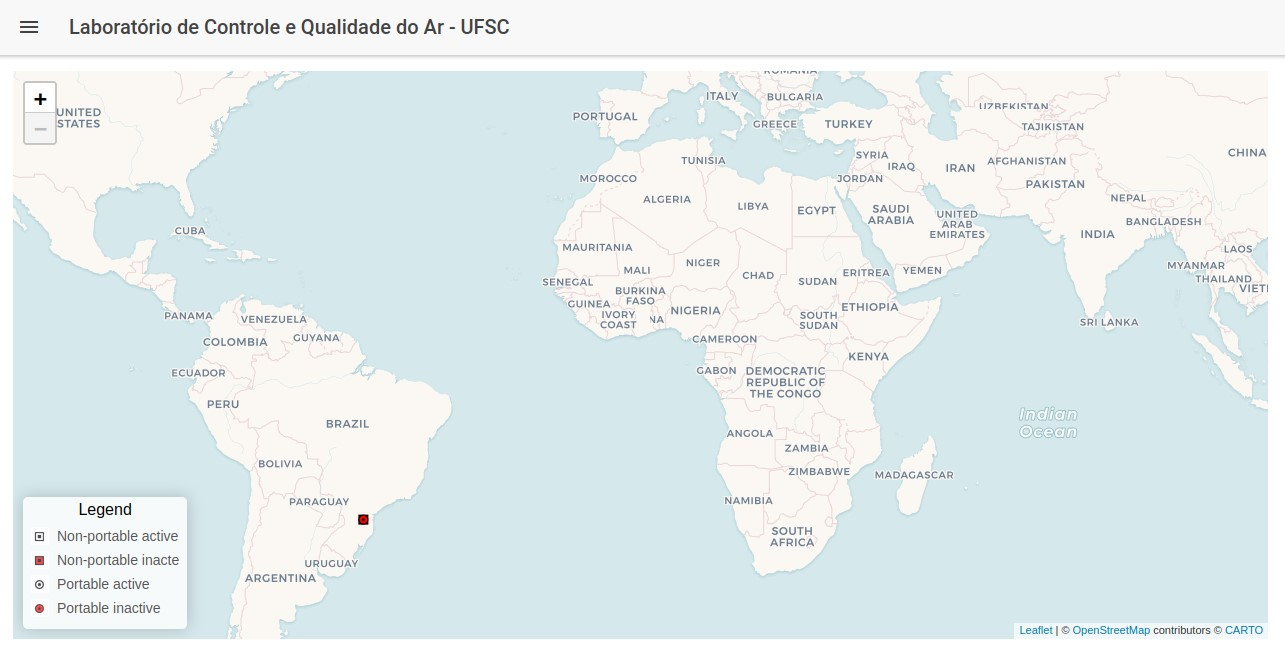
\includegraphics[width=\textwidth]{chapters/2-CLEAN/Figuras/Renovar main panel.jpeg}
        \caption{Painel principal}
        \label{fig:renovar-map}
    \end{subfigure}
    \hfill
    \begin{subfigure}{0.495\textwidth}
        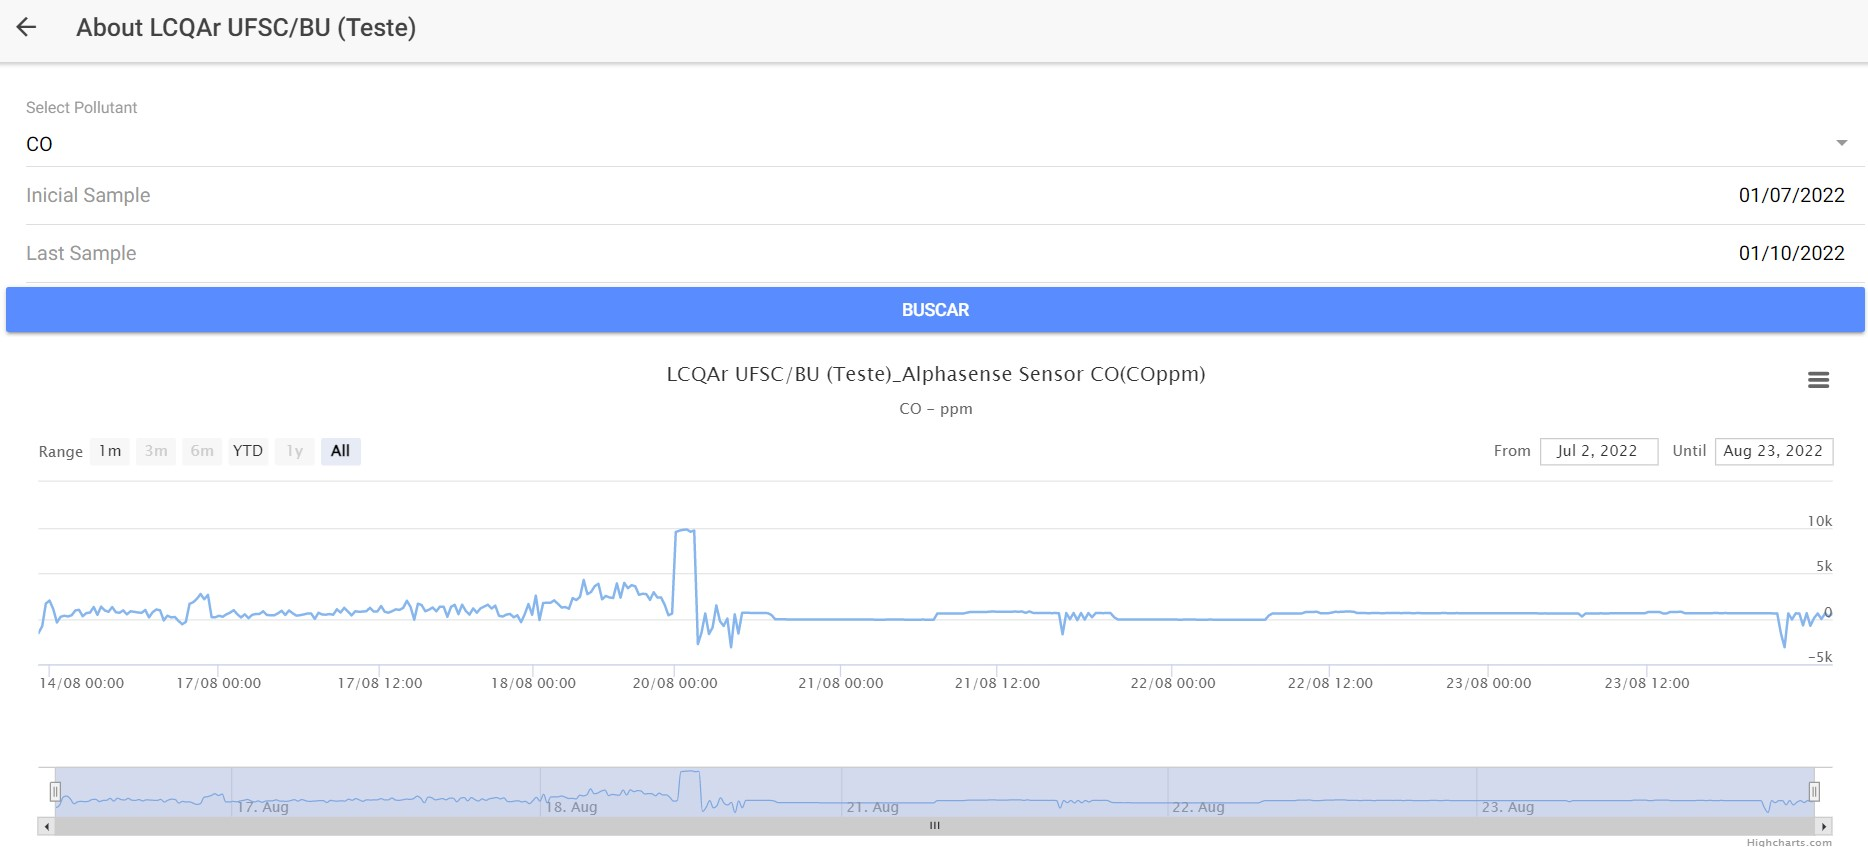
\includegraphics[width=\textwidth]{chapters/2-CLEAN/Figuras/ Renovar time series panel.jpg}
        \caption{Painel de visualização de séries temporais}
        \label{fig:renovar-series}
    \end{subfigure}
    \hfill
    \label{fig:renovar-map-and-series}
    \fonte{Desenvolvido pelo autor (2023)}
\end{figure}

O sistema recebe dados de dispositivos \acrshort{iot}, como concentração de poluentes atmosféricos, temperatura e umidade relativa. Os dados são armazenados em um banco de dados como séries temporais que podem ser visualizadas online na plataforma \textit{web}. O software consiste em (1) um banco de dados MySQL que armazena as leituras do dispositivo e demais dados necessários à plataforma, como usuários, dispositivos cadastrados, poluentes e unidades; (2) um back-end RESTful, desenvolvido em Java utilizando Spring Boot, que é responsável por coletar dados do banco de dados e prepará-los para o frontend; e (3) o front-end, desenvolvido para ser multiplataforma, disponibilizando a interface com o usuário conforme ilustrado nas imagens da Figura \ref{fig:renovar-map-and-series}. O banco de dados, backend e frontend estão hospedados em um servidor da Universidade Federal de Santa Catarina.

\begin{figure}[h]
    \centering
    \caption{Estrutura da aplicação \textit{Web} Renovar}
    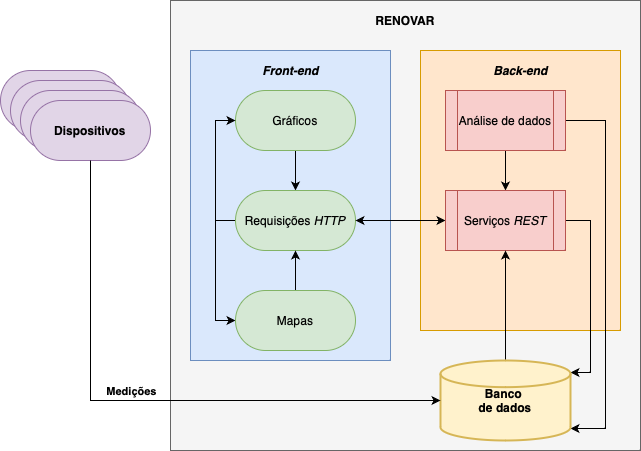
\includegraphics[width=0.80\linewidth]{chapters//2-CLEAN/Figuras/Renovar Structure (PT).png}
    \label{fig:renovar-structure}
    \fonte{Desenvolvido pelo autor (2023)}
\end{figure}

A Figura \ref{fig:renovar-structure} ilustra o funcionamento do serviço em geral. Os dispositivos coletam dados ambientais e os enviam para o banco de dados pela internet. O backend recebe solicitações do frontend e coleta os dados necessários do banco de dados. Caso os dados necessitem de algum tratamento (ex.: cálculo de valores médios ou filtragem), o backend executa as operações necessárias e envia as informações processadas de volta ao frontend. O frontend, por outro lado, implementa a interface com o usuário e gera os resultados das operações solicitadas, como visualizar os dados como séries temporais e baixar os dados como arquivo \acrshort{csv}.

\subsection{Banco de dados}

O banco de dados foi construído utilizando \textit{MySQL} como linguagem de consulta e \textit{phpMyAdmin} para administração. A Figura \ref{fig:renovar-database} ilustra a estrutura do banco, que consiste em oito entidades, cada uma com a sua função, atributos e relacionamentos. Elas são as entidades \textit{User}, \textit{Device}, \textit{Sensor}, \textit{Sample}, \textit{Coordinates}, \textit{Pollutant}, \textit{Unit} e \textit{Type}.

\begin{figure}[h]
    \centering
    \caption{Entidades do banco de dados Renovar}
    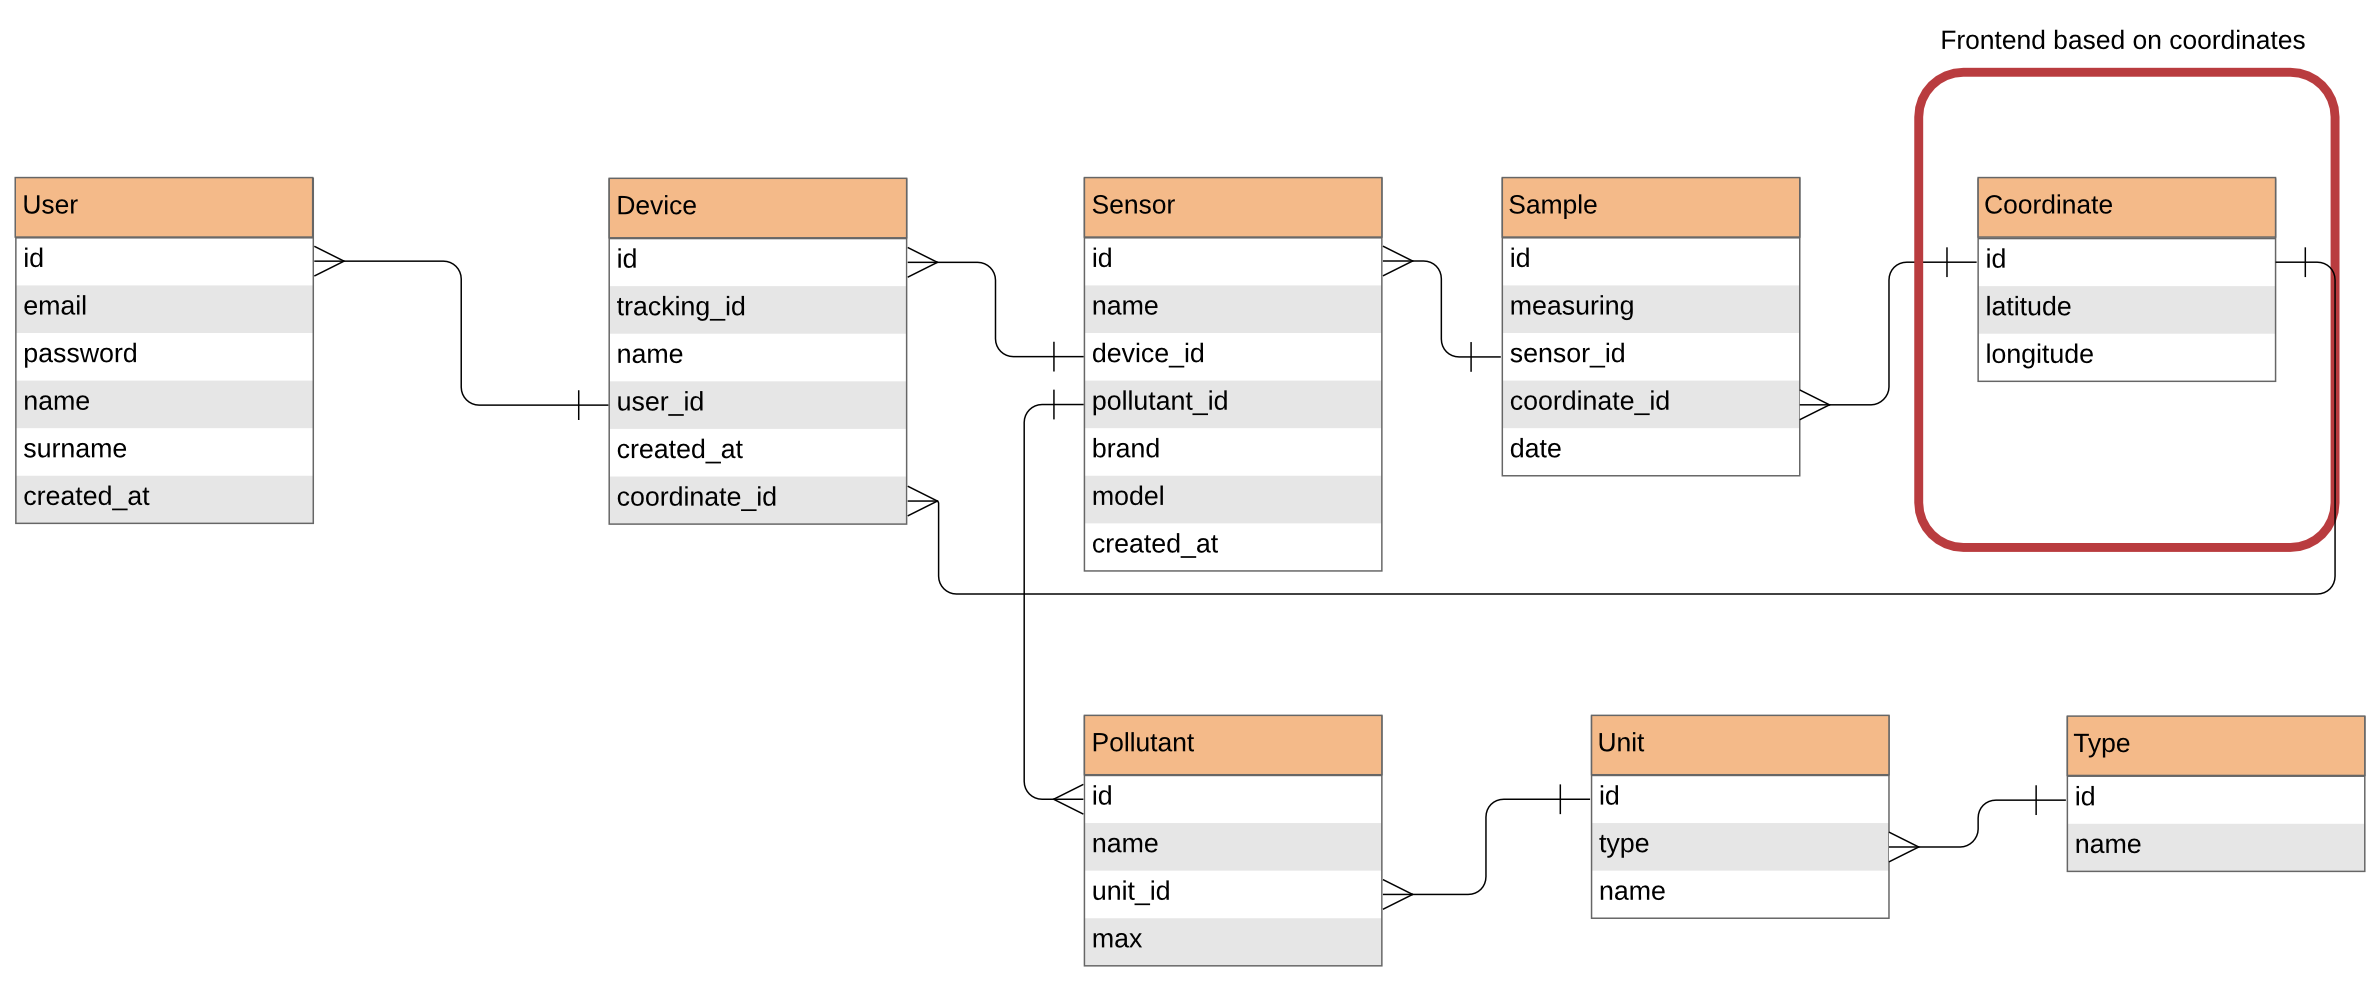
\includegraphics[width=0.80\linewidth]{chapters//2-CLEAN/Figuras/Renovar Database.png}
    \label{fig:renovar-database}
    \fonte{Desenvolvido pelo autor (2023)}
\end{figure}

A entidade \textit{Device} representa na prática os dispositivos de coleta, mais especificamente os monitores de qualidade do ar. A entidade \textit{Sensor} representa um sensor de determinada variável física. Relaciona-se com a entidade \textit{Device} com uma cardinalidade 1:N, ou seja, um dispositivo pode ter N sensores enquanto um sensor pode pertencer apenas a um dispositivo. \textit{Pollutant} representa as variáveis que são monitoradas no meio ambiente pelos dispositivos \acrshort{iot}. A relação entre \textit{Pollutant} e \textit{Sensor} também está caracterizada por uma cardinalidade 1:N, já que um sensor possui um único poluente, mas um mesmo poluente pode estar associado a N sensores. Cada poluente tem associado também uma unidade de medida e um tipo de unidade. A entidade \textit{Sample} representa uma leitura de determinada variável física; existem N amostras por sensor. Cada amostra tem associada uma coordenada, que é a localização geográfica onde o valor da amostra será mostrado no mapa. Os dispositivos para medição em locais fixos também tem associados uma Coordenada e consequentemente, todas as amostras dos sensores desse dispositivo devem possuir os mesmos valores de latitude e longitude. Por último, a entidade \textit{User} é utilizada para controle de acesso à plataforma. Embora o acesso aos dados de Renovar não precise de uma etapa de login, a escrita ou envio de dados para a plataforma precisa de um cadastro prévio. Assim, cada dispositivo deve ter um usuário associado para conseguir armazenar as leituras no banco de dados de Renovar.

\subsection{A aplicação \textit{Back-end}}

O backend é uma aplicação autônoma construída na linguagem de programação \textit{Java}, com o \textit{framework Spring Boot} e a ferramenta \textit{Maven}. Esta aplicação é responsável por receber e organizar as leituras enviadas pelos dispositivos \acrshort{iot}, no banco de dados e atender as requisições \textit{HTTP} do lado do cliente (\textit{front-end}). Igualmente a aplicação realiza algumas operações básicas de análise de dados como filtragem e agrupação para gráficos tipo \textit{box-plots}.

Quatro camadas compõem a aplicação: os controladores \acrshort{rest}, a camada de serviço, a camada de acesso aos dados e a camada de domínio (Figura \ref{fig:renovar-backend}) \cite{Teixeira2018}. São os controladores os que estabelecem os \textit{endpoints}, mensagens, conteúdos e cabeçalhos de cada recurso do \textit{back-end}. A Camada de Serviço está abaixo dos controladores \acrshort{rest} e funciona como um mediador entre a Camada de Acesso aos Dados e a Camada de Comunicação. É ela também quem define as regras de negócio da aplicação. A Camada de Domínio replica a modelagem do banco de dados em classes que são utilizadas pelos distintos componentes da aplicação; cada classe representa uma tabela. Por último a Camada de Acesso aos Dados tem a responsabilidade de acessar diretamente o banco de dados e disponibilizar a informação para as camadas superiores. A Figura \ref{fig:renovar-backend-dao} ilustra as classes utilizadas na Camada de Acesso aos Dados.

\begin{figure}[h]
    \centering
    \caption{Camadas da aplicação \textit{back-end} Renovar}
    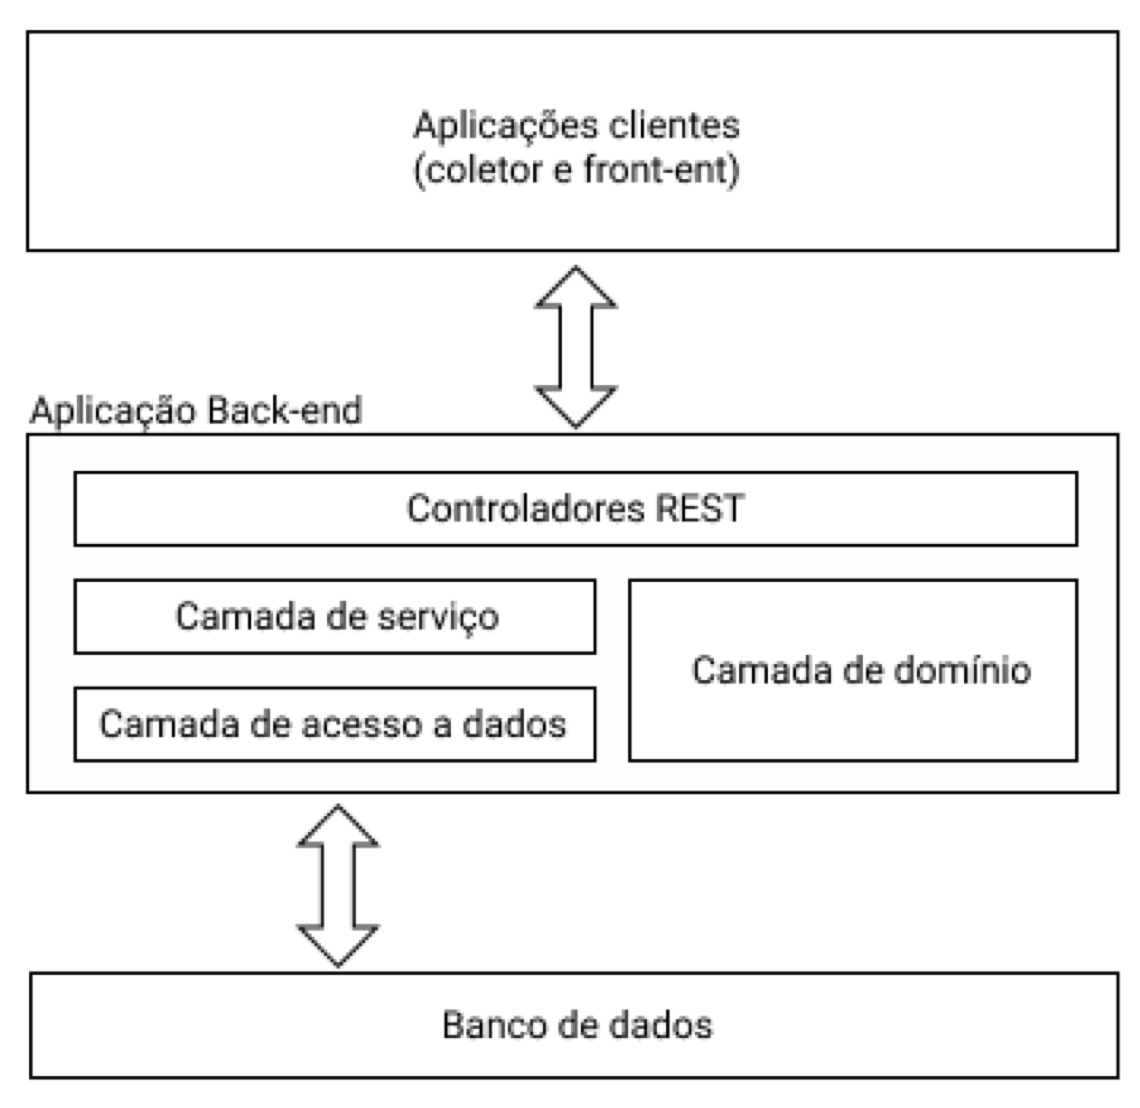
\includegraphics[width=0.80\linewidth]{chapters//2-CLEAN/Figuras/Renovar back-end strcuture.png}
    \label{fig:renovar-backend}
    \fonte{\cite{Teixeira2018}}
\end{figure}

\begin{figure}[h]
    \centering
    \caption{Classes de acesso ao dados da aplicação \textit{back-end} Renovar}
    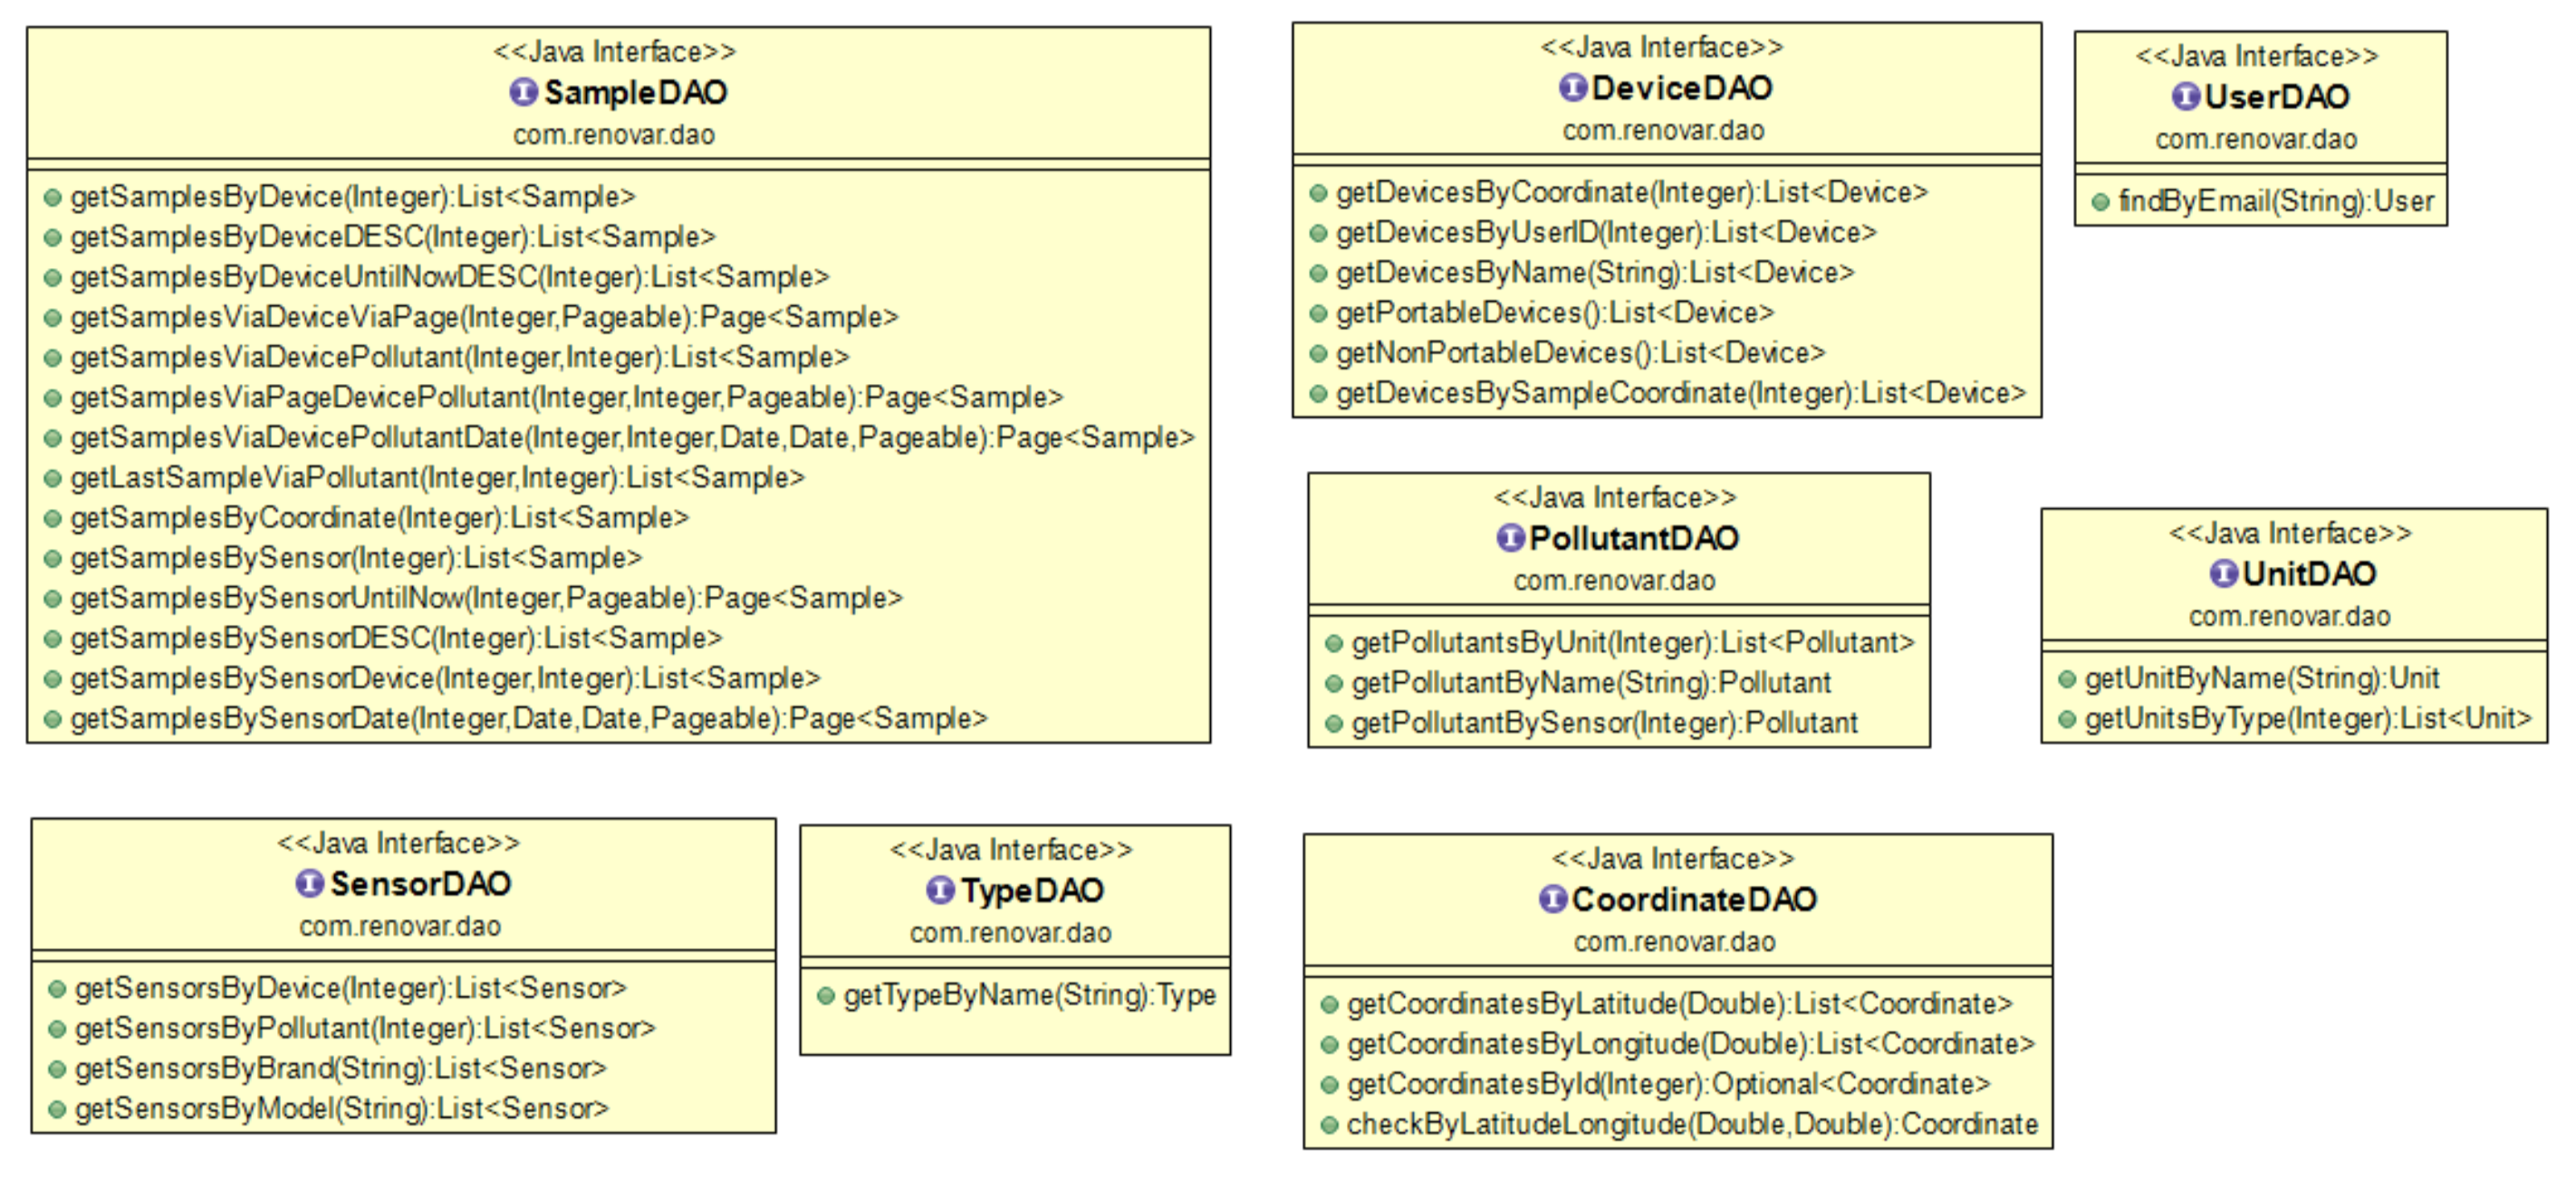
\includegraphics[width=0.80\linewidth]{chapters//2-CLEAN/Figuras/Classes de acesso aos Dados.png}
    \label{fig:renovar-backend-dao}
    \fonte{Desenvolvido pelo autor (2023)}
\end{figure}

O processo de coleta das medições enviadas pelos dispositivos de monitoramento na aplicação \textit{back-end} consiste, de forma simplificada, no seguinte fluxo de execução. Os controladores \acrshort{rest} processam as requisições de tipo \textit{POST HTTP} enviadas pelos dispositivos \acrshort{iot}, e transferem as informações até a camada de serviço. Ali os dados são validados e instâncias da entidade \textit{Sample} são criadas e transferidas até a camada de acesso aos dados onde as amostras são armazenadas na tabela correspondente do banco de dados. As requisições e os \textit{endpoints} disponibilizados na \acrshort{api} Renovar pelos controladores \acrshort{rest} são detalhados na documentação da \acrshort{api} disponibilizada no Anexo \ref{anex:renovar-api}.

\subsection{A aplicação \textit{Front-end}}

A aplicação \textit{front-end} foi construída usando o \textit{framework Angular}, junto com outras ferramentas como \textit{HighCharts} e \textit{HighStock} para os gráficos e \textit{Leaflet} para mapas. A tela principal mostra um mapa com todos os dispositivos (Figura \ref{fig:renovar-map-2}). A cor dos dispositivos no mapa indica seu estado: verde para ativo (i.e.: o dispositivo está transmitindo novas medidas), vermelho para inativo (o dispositivo não tem enviado novas medidas em um determinado intervalo de tempo). Quando o usuário seleciona um dispositivo no mapa, um \textit{pop-up} é aberto com informações sobre esse e todos os dispositivos que se encontrem nas mesmas coordenadas geográficas, juntamente com informações sobre seus sensores (Figura \ref{fig:renovar-devices}). A partir desse ponto, o usuário pode acessar a página do dispositivo e escolher um poluente para visualizar sua série histórica dentro de um intervalo de datas (Figura \ref{fig:renovar-series-2}). Se o aparelho for portátil, o usuário também pode ver outro mapa que mostra onde cada amostra foi coletada, conforme mostrado na Figura \ref{fig:renovar-portable-map}. Uma seção de análise de dados possibilita visualizar os valores das leituras dos sensores em gráficos de \textit{box-plots}, agrupando as medições por ano mês ou semana, conforme ilustra a Figura \ref{fig:renovar-data-analysis}.

\begin{figure}[h]
    \centering
    \caption{Aplicação \textit{front-end} da plataforma web Renovar}
    \begin{subfigure}{0.495\textwidth}
        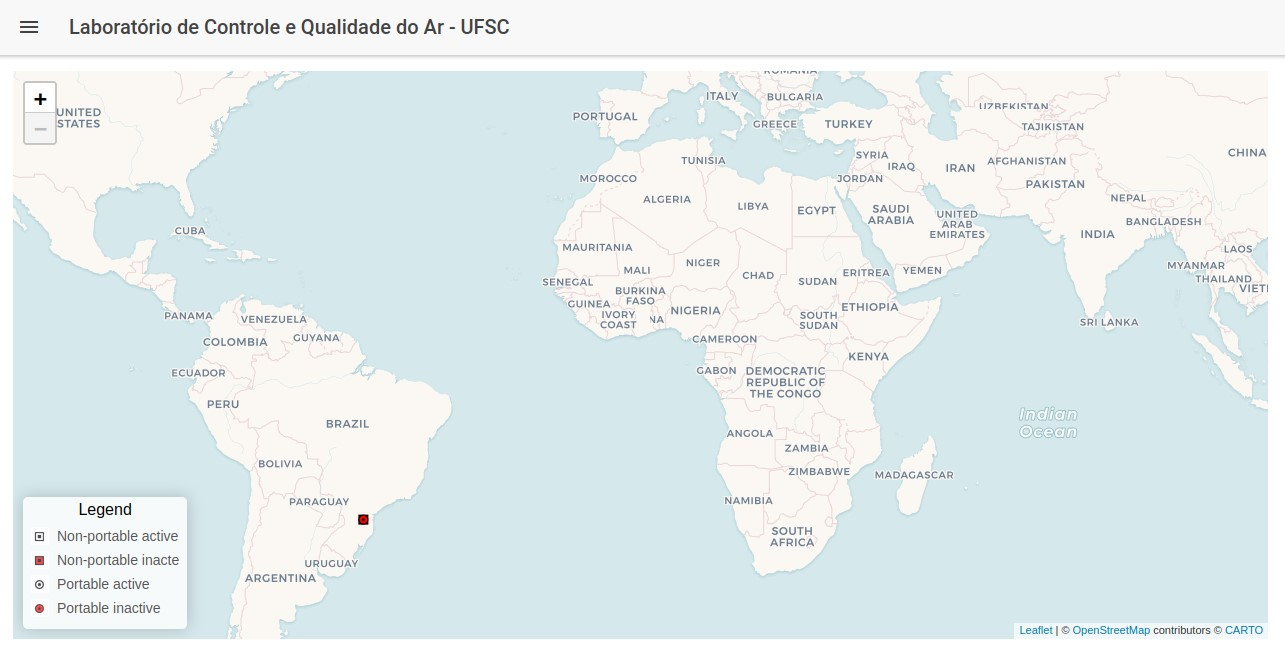
\includegraphics[width=\textwidth]{chapters/2-CLEAN/Figuras/Renovar main panel.jpeg}
        \caption{Mapa de dispositivos}
        \label{fig:renovar-map-2}
    \end{subfigure}
    \hfill
    \begin{subfigure}{0.495\textwidth}
        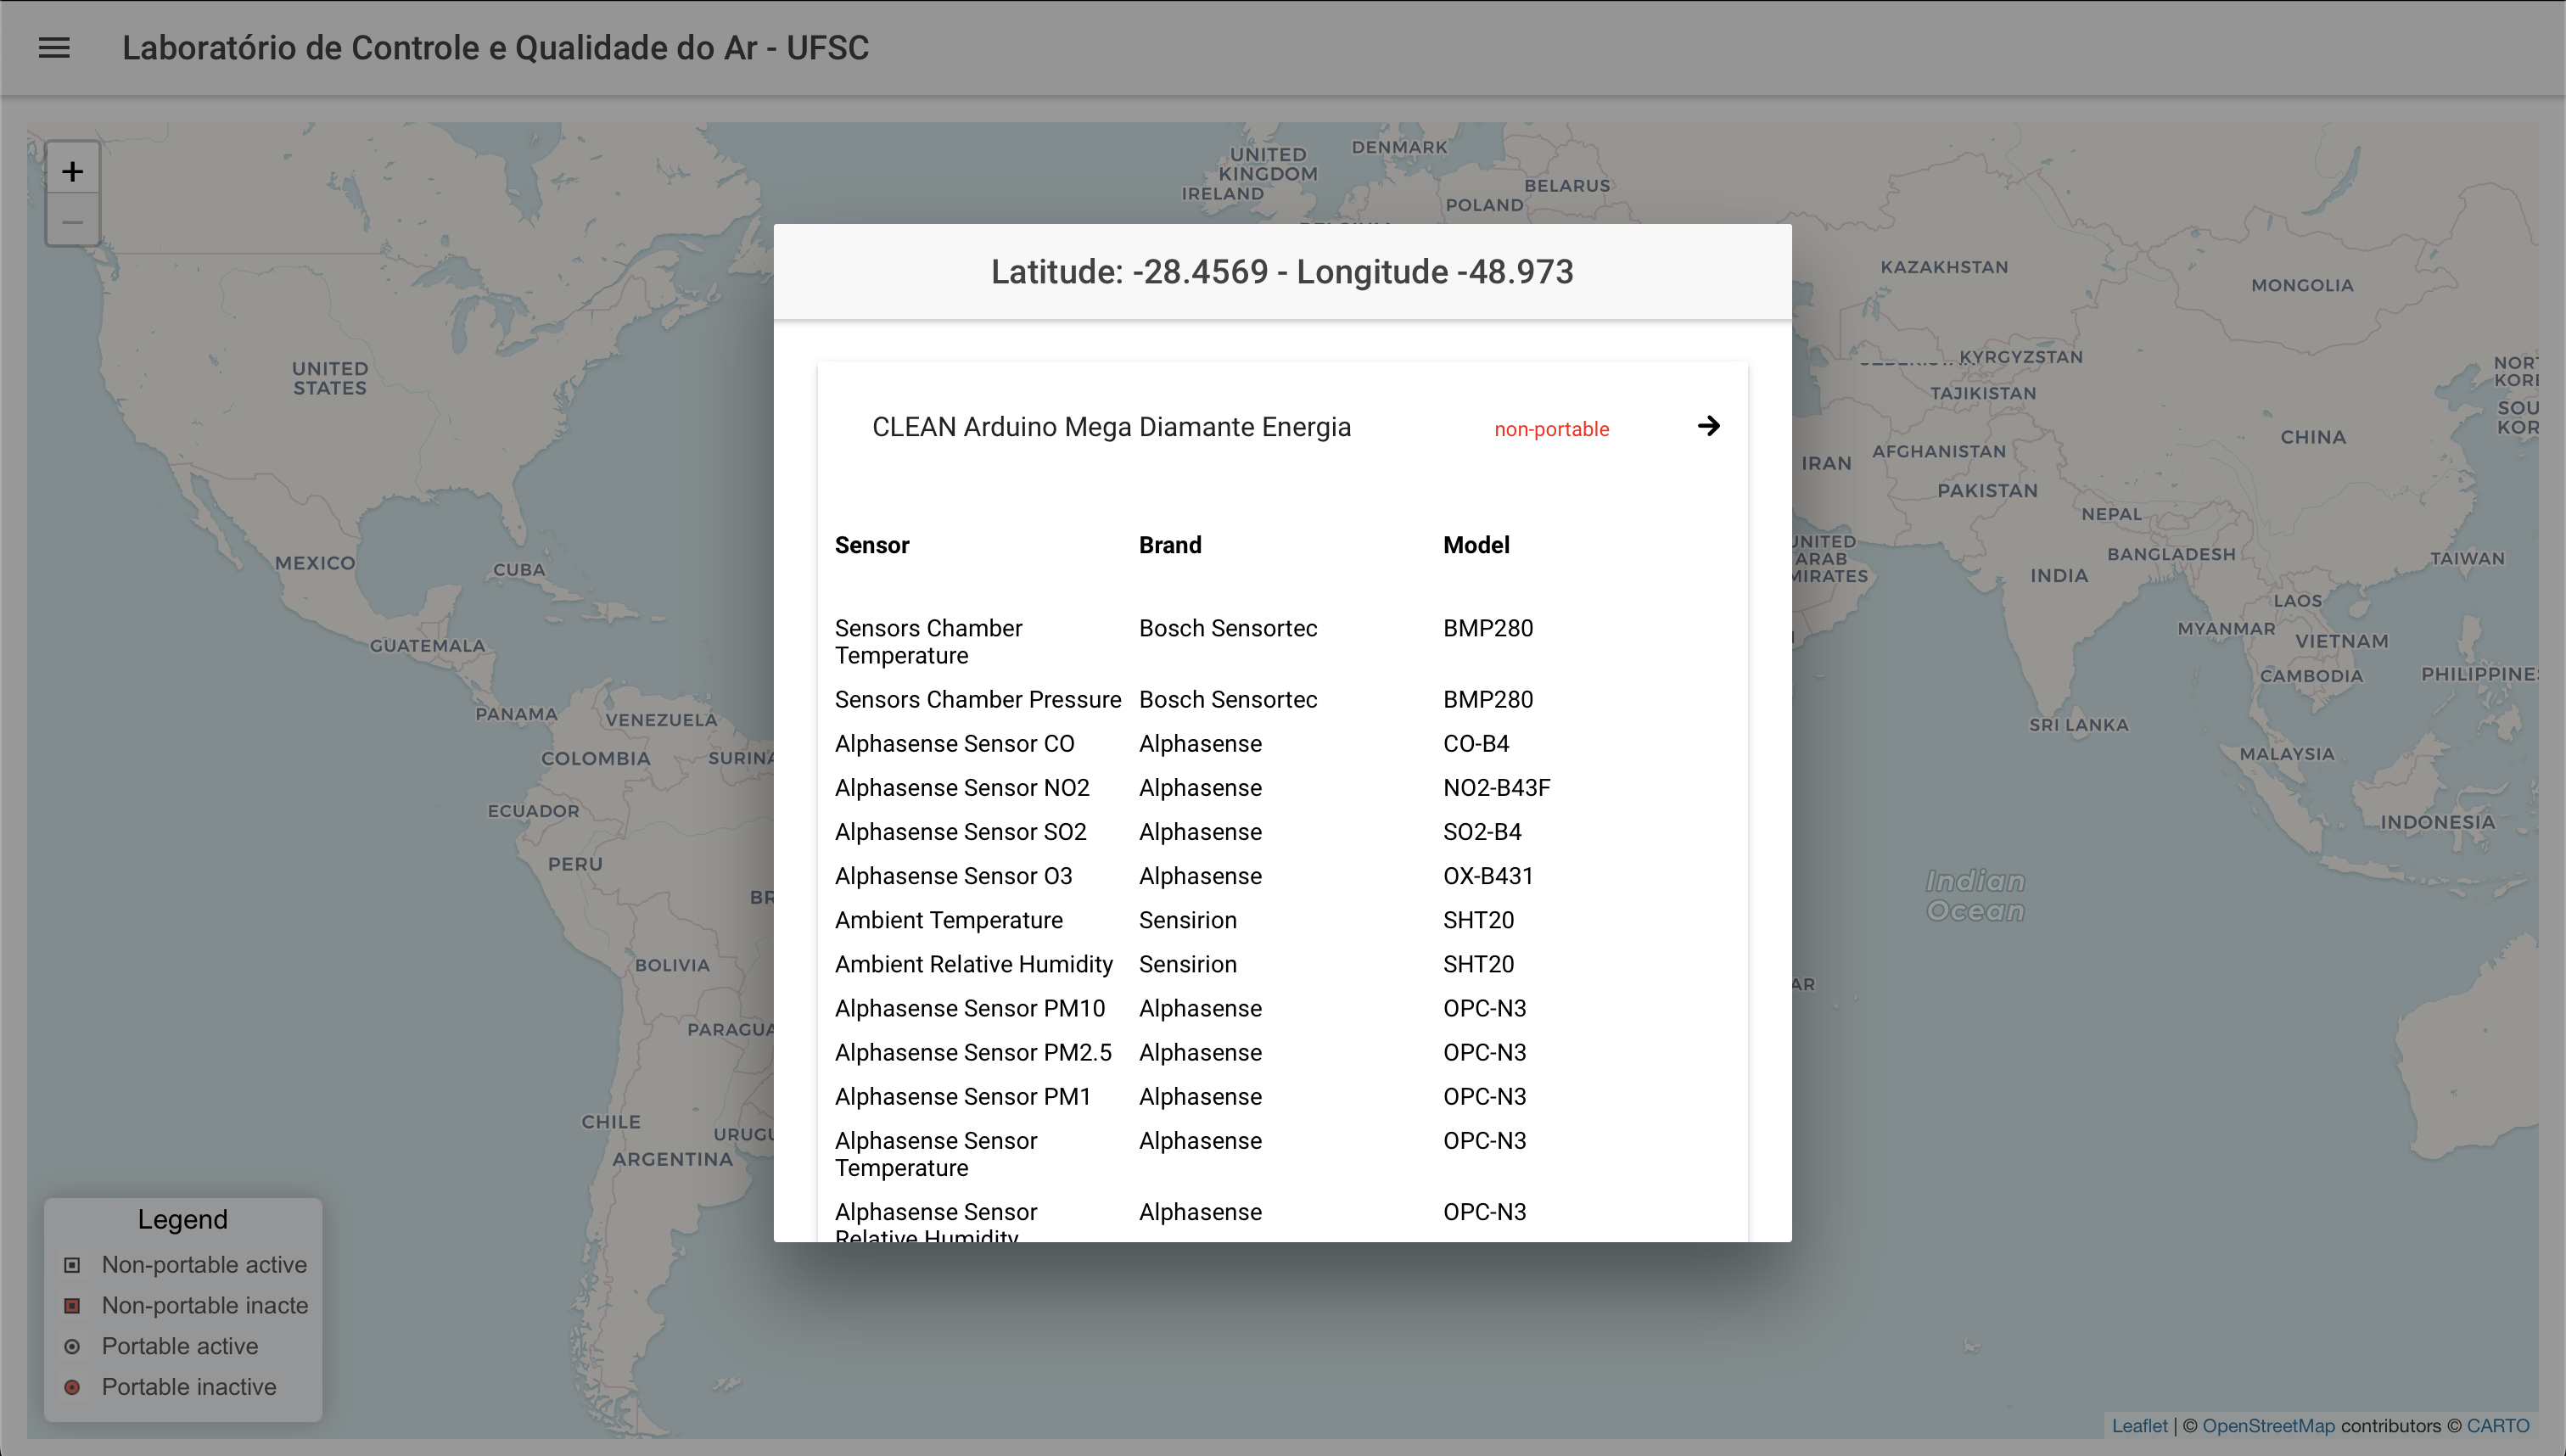
\includegraphics[width=\textwidth]{chapters/2-CLEAN/Figuras/Renovar Device Information.png}
        \caption{Painel de seleção de dispositivos}
        \label{fig:renovar-devices}
    \end{subfigure}
    \hfill
    \label{fig:renovar-map-and-devices}
    \fonte{Desenvolvido pelo autor (2023)}
\end{figure}

\begin{figure}[h]
    \centering
    \caption{Painéis da aplicação \textit{front-end} de Renovar}
    \begin{subfigure}{0.495\textwidth}
        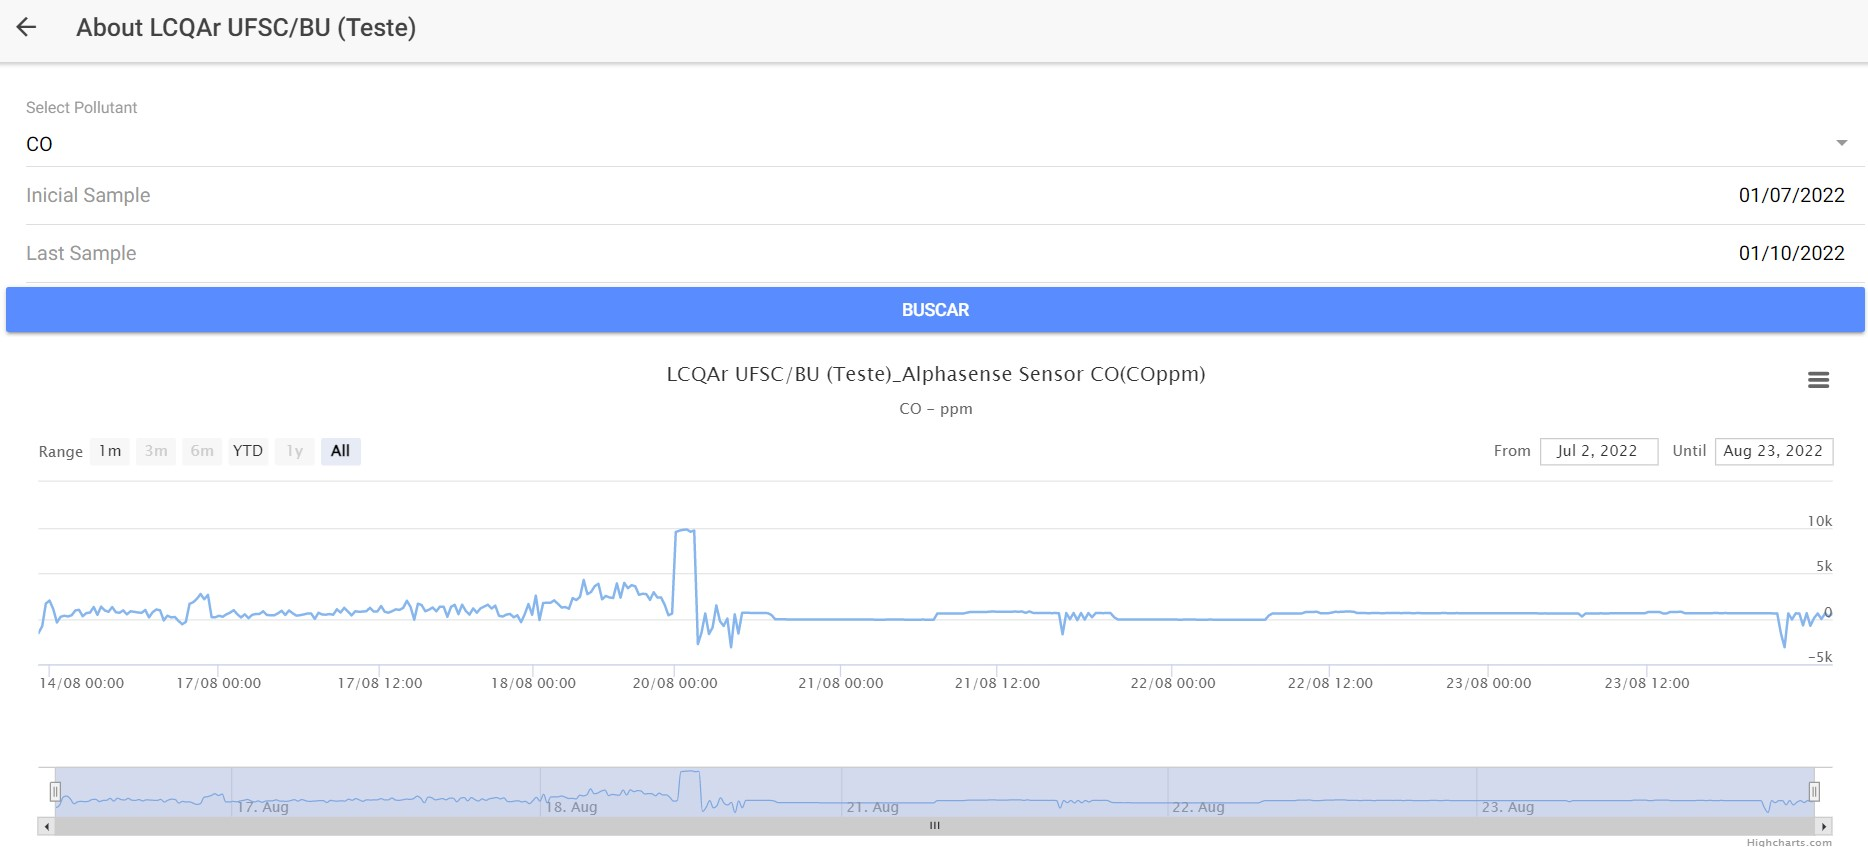
\includegraphics[width=\textwidth]{chapters/2-CLEAN/Figuras/ Renovar time series panel.jpg}
        \caption{Mapa de dispositivos}
        \label{fig:renovar-series-2}
    \end{subfigure}
    \hfill
    \begin{subfigure}{0.495\textwidth}
        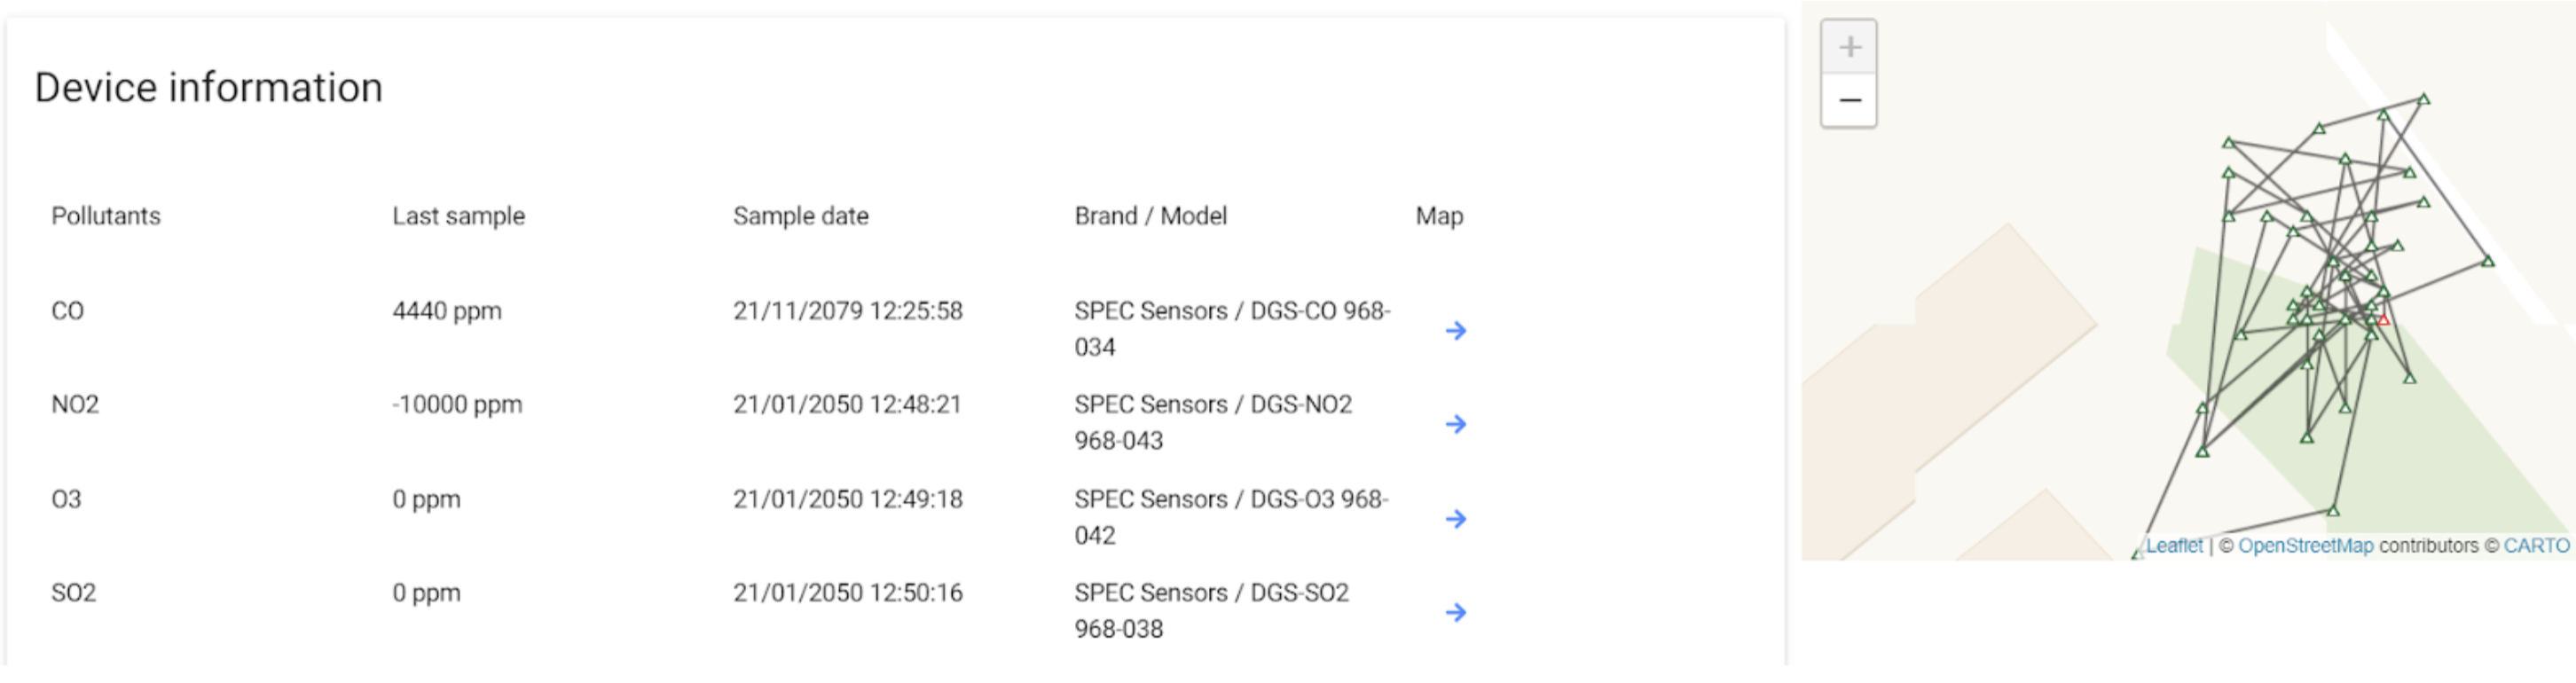
\includegraphics[width=\textwidth]{chapters/2-CLEAN/Figuras/Renovar portable map.png}
        \caption{Painel de seleção de dispositivos}
        \label{fig:renovar-portable-map}
    \end{subfigure}
    \hfill
    \label{fig:renovar-series-and-map}
    \fonte{Desenvolvido pelo autor (2023)}
\end{figure}

\begin{figure}[h]
    \centering
    \caption{Painel de análise de dados da aplicação \textit{back-end} Renovar}
    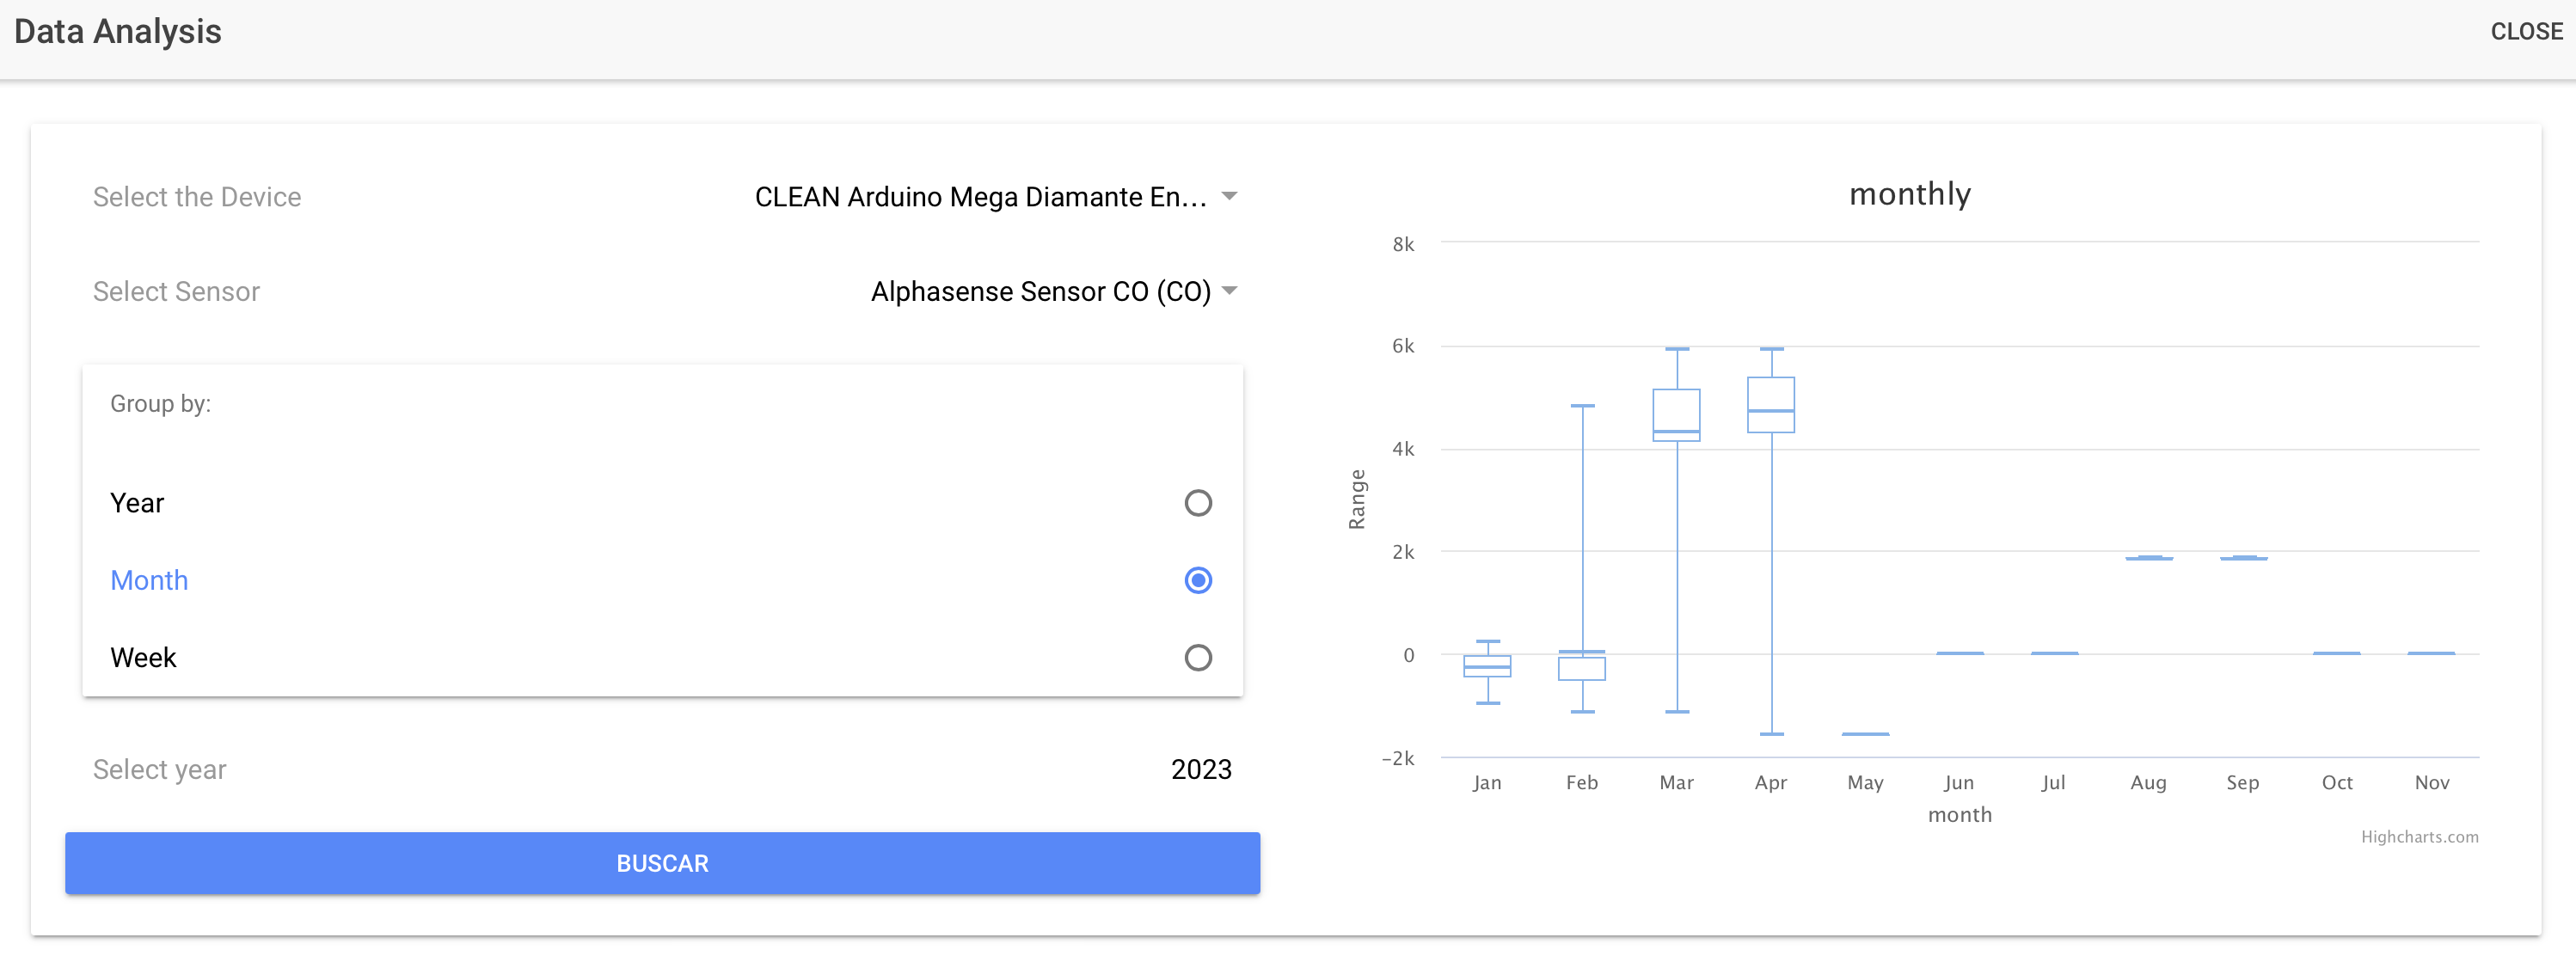
\includegraphics[width=0.80\linewidth]{chapters//2-CLEAN/Figuras/Renovar Data Analysis Panel.png}
    \label{fig:renovar-data-analysis}
    \fonte{Desenvolvido pelo autor (2023)}
\end{figure}